\chapter{前言}
\renewcommand{\baselinestretch}{10.0} %設定行距
\pagenumbering{arabic} %設定頁號阿拉伯數字
\setcounter{page}{1}  %設定頁數
\fontsize{14pt}{2.5pt}\sectionef
\section{研究動機}
機器學習與各領域結合的應用越來越廣泛,在機電系統採用強化學習是為了讓機電系統的控制達到最佳化。本專題以實體的足球機之機電系統作為訓練模型,將實體機器轉移到虛擬環境進行模擬,為了找到適合的訓練參數,因此將模型簡化後再進行測試各種參數的優劣,透過不斷的訓練來得到一個優化過的對打系統,以下是成品圖。\\

\begin{figure}[hbt!]
\begin{center}
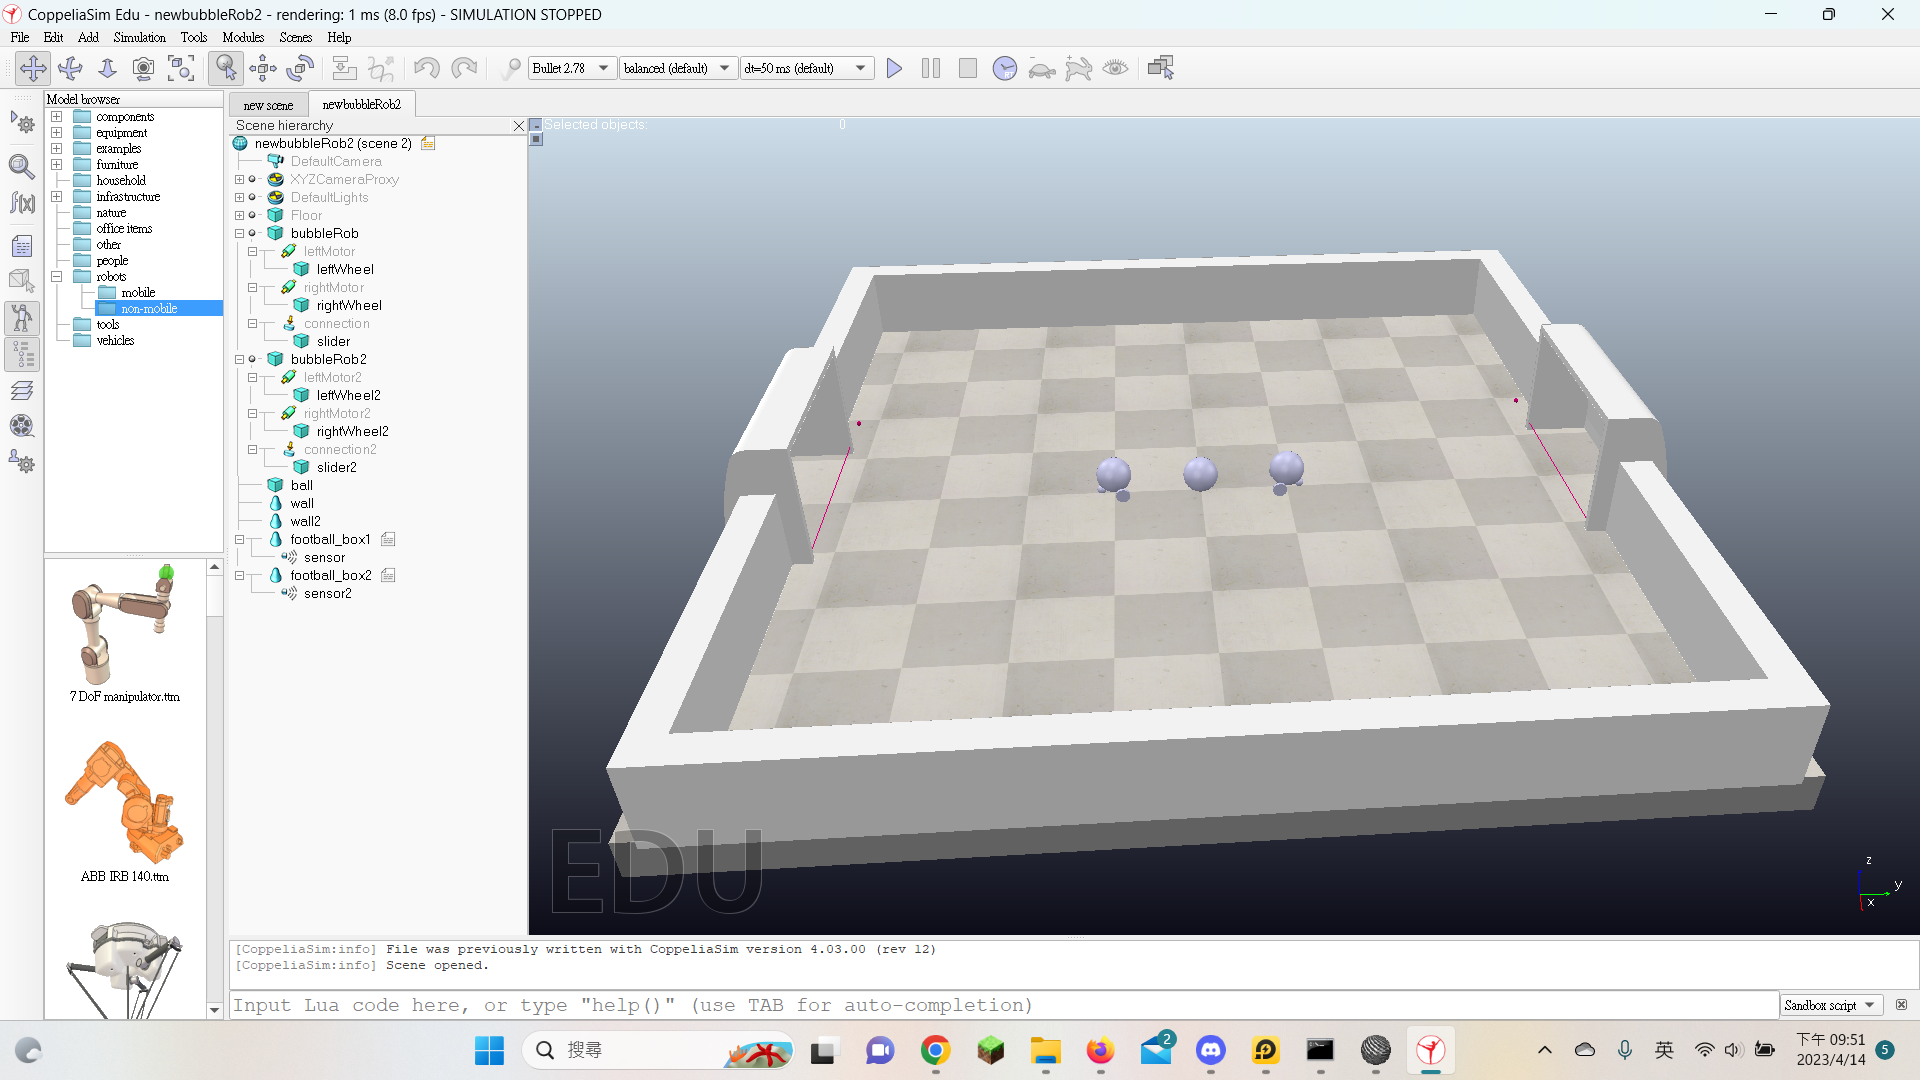
\includegraphics[angle=0,width=17cm]{2023-04-14}
\end{center}
\end{figure}
